\documentclass[25pt, a0paper, portrait, margin=0mm, innermargin=20mm,
blockverticalspace=2mm, colspace=20mm, subcolspace=0mm]{tikzposter} %Default values for poster format options.

\usepackage[utf8]{inputenc}
\usepackage[scaled]{helvet}
\renewcommand\familydefault{\sfdefault} 
\usepackage[T1]{fontenc}
\usepackage{wrapfig}
\usepackage{setspace}
\usepackage{multicol}
\setlength{\columnsep}{1.5cm}
\usepackage{xspace}
\usepackage{tikz}
\tikzposterlatexaffectionproofoff
\usetheme{Default}

\definecolor{unired}{HTML}{a51e37}
\definecolor{mypink1}{rgb}{0.858, 0.188, 0.478}
\definecolor{mblack}{HTML}{0d0d0d}
\definecolor{titlecolor}{RGB}{74, 114, 159}
\definecolor{titledarkcolor}{RGB}{51,102,153}
\definecolor{Grey}{HTML}{e1e1e1}
\definecolor{DarkerGrey}{RGB}{215,217,219}
\definecolor{FontColor}{HTML}{0d0d0d}
\definecolor{Red}{RGB}{204,0,0}
\definecolor{L-lig}{RGB}{25,124,192}
\definecolor{point-lig}{RGB}{255,255,255}
\definecolor{G-lig}{RGB}{62,66,68}

\definecolor{Orange}{RGB}{240,163,10} 
\definecolor{LightRed}{RGB}{214,98,93}
\definecolor{LightBlue}{RGB}{160,200,217}
\definecolor{LightGreen}{RGB}{130,161,119}
\definecolor{Violet}{RGB}{190,144,252}

\colorlet{blocktitlefgcolor}{mblack}
\colorlet{backgroundcolor}{Grey}
\colorlet{blocktitlebgcolor}{Grey}
\colorlet{blockbodyfgcolor}{FontColor}
\colorlet{innerblocktitlebgcolor}{L-lig}
\colorlet{innerblocktitlefgcolor}{white}
\colorlet{notefrcolor}{white}
\colorlet{notefgcolor}{black}
\colorlet{notebgcolor}{white}


% Title setup
\settitle{ 
\begin{minipage}[b]{0.8\linewidth}
\vspace{2cm}
\hspace{1cm}\color{mblack}{ \Huge{\textbf{\@title}} \par } \vspace*{2em} \hspace{1cm}\color{mblack}{\LARGE \@author \par} \vspace*{2em} \hspace{1cm}{\Large \@institute}\vspace{0.5cm} \end{minipage}

% Add institution logo
\hfill
\begin{minipage}[t]{0.2\linewidth}
    \vspace{-13.8cm}\hspace{-3.8cm}
    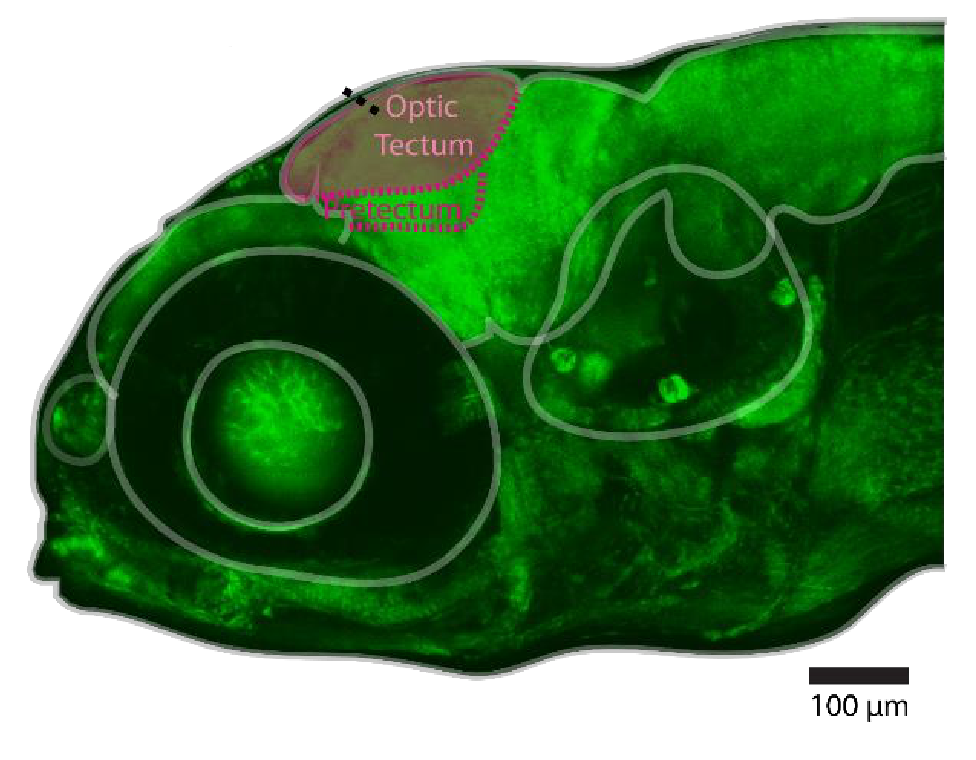
\includegraphics[width=13cm]{figs/titlepic.png} 
\end{minipage}}

% define title style with background box (currently white)
\definetitlestyle{sampletitle}{
width=841mm, roundedcorners=0, linewidth=0pt, innersep=15pt,
titletotopverticalspace=0mm, titletoblockverticalspace=5pt
}{\begin{scope}[line width=\titlelinewidth, rounded corners=\titleroundedcorners]\draw[fill=point-lig, color=point-lig]
(\titleposleft,\titleposbottom) rectangle (\titleposright,\titlepostop);
\end{scope}}

 % Title, Author, Institute
\title{\parbox{1500pt}{Complex frequency modulations in freely interacting electric fish, \textit{Apteronotus leptorynchus}, recorded in their natural habitat}}
\author{Patrick Weygoldt, Till Raab, Jan Benda}
\institute{Neuroethology Lab, Department of Neurobiology, University of Tuebingen}
\usetitlestyle[]{sampletitle}

% define coustom block style
\defineblockstyle{MyBlock}{% define a custom style for a block
    titlewidthscale=1, bodywidthscale=1, titlecenter,
    titleoffsetx=0pt, titleoffsety=-30pt, bodyoffsetx=0pt, bodyoffsety=-40pt,
    bodyverticalshift=0mm, roundedcorners=25, linewidth=1pt,
    titleinnersep=20pt, bodyinnersep=38pt
}{
    \draw[rounded corners=\blockroundedcorners, inner sep=\blockbodyinnersep,
          line width=\blocklinewidth, color=white,
          top color=titlebgcolor!90, bottom color=titlebgcolor!20!white,
          ]
      (blockbody.south west) rectangle (blockbody.north east); %
    \ifBlockHasTitle%
        \draw[rounded corners=\blockroundedcorners, inner sep=\blocktitleinnersep,
          top color=Grey, bottom color=Grey,
          line width=2, color=Grey, %fill=blocktitlebgcolor
          ]
      (blocktitle.south west) rectangle (blocktitle.north east); %
    \fi%
}
\newcommand\myblock[3][MyBlock]{\useblockstyle{#1}\block{#2}{#3}\useblockstyle{Default}}

\begin{document}
 
\renewcommand{\baselinestretch}{1} 
\title{\parbox{1500pt}{Motion blindness induced by color in zebrafish larvea \textit{Danio rerio}}}
\author{Alexander Wendt, Patrick Weygoldt}
\institute{Systems Neurobiology, Department of Neurobiology, University of Tuebingen}
\usetitlestyle[]{sampletitle}
\maketitle
\renewcommand{\baselinestretch}{1.4} 

\begin{columns}
\column{0.3333}
\myblock[MyBlock]{Introduction}{
   Color has a big influence on motion vision in zebrafish. 
   Michael B. Orger (2004) displayed that zebrafish in behavioural experiments show motion blindness 
   to a grating of different colors, but little is known about the cortical structures conveing the
   \glqq color-motion\grqq{} perception. We wanted to the investigate the 
   optic tectum of the zebrafish larvae with calcium imaging. 
    
   \vspace{0.6cm}
        \begin{tikzfigure}[]
            \label{Rois}
            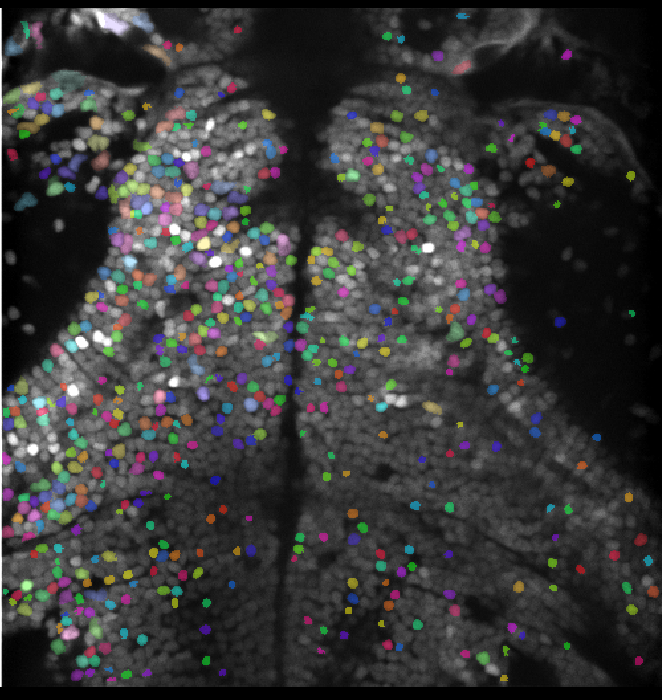
\includegraphics[width=8cm]{figs/Screenshot 2022-11-17 at 19.05.14.png}
        \end{tikzfigure} 
}

\myblock[MyBlock]{Preprocessing:}{
    \textbf{1. Region of Interests (ROI):} corrosponds to neurons with 
    genetically encoded caclium indicators. The lumiance $f$ of the calcium imaging is calculated from the change of luminance normalized to the average luminance $f = \frac{\Delta f}{f}$.   
    
    \vspace{0.6}

    \begin{tikzfigure}[]
        \label{Raw}
        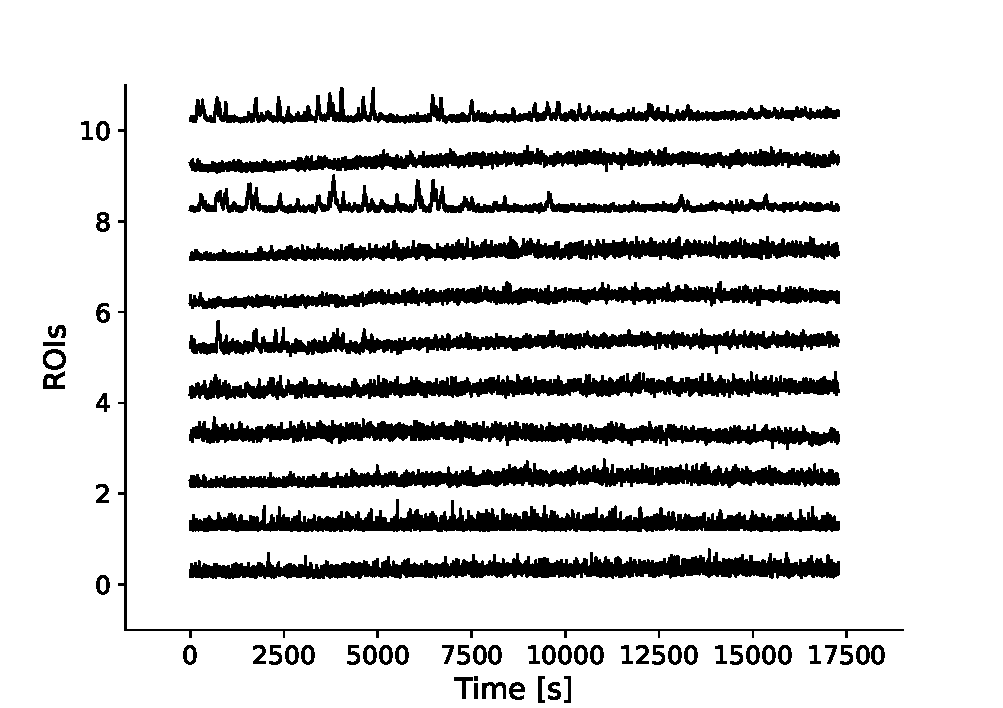
\includegraphics[width=24cm]{figs/raw2.pdf}
    \end{tikzfigure} 

    \vspace{0.6cm}
    \textbf{2. Active ROIs:}
    To get the active ROIs we computed the correlation within 3 repeats of the same stimulus.  
    \vspace{0.6}

    \begin{minipage}{0.08\textwidth}
    \begin{tikzfigure}[]
        \label{Rois}
        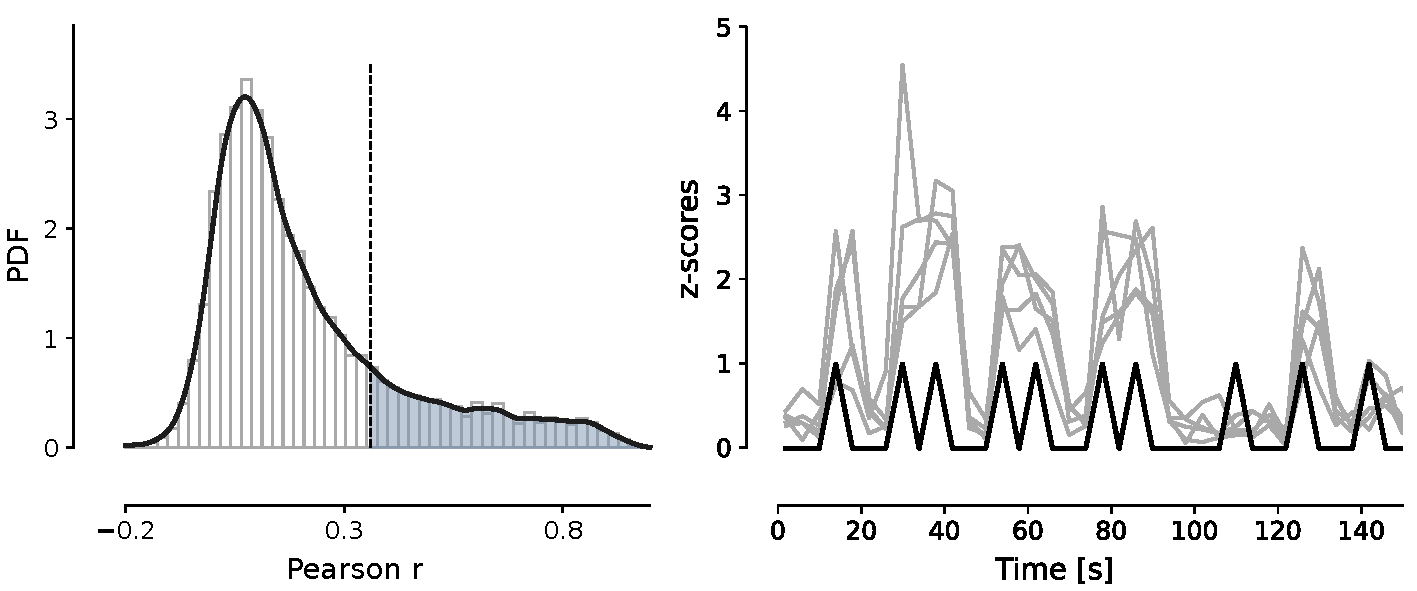
\includegraphics[width=10cm]{figs/pcorrelation.pdf}
    \end{tikzfigure} 
    \end{minipage}
    \begin{minipage}{0.24\textwidth}
    \begin{tikzfigure}[]
        \label{Raw}
        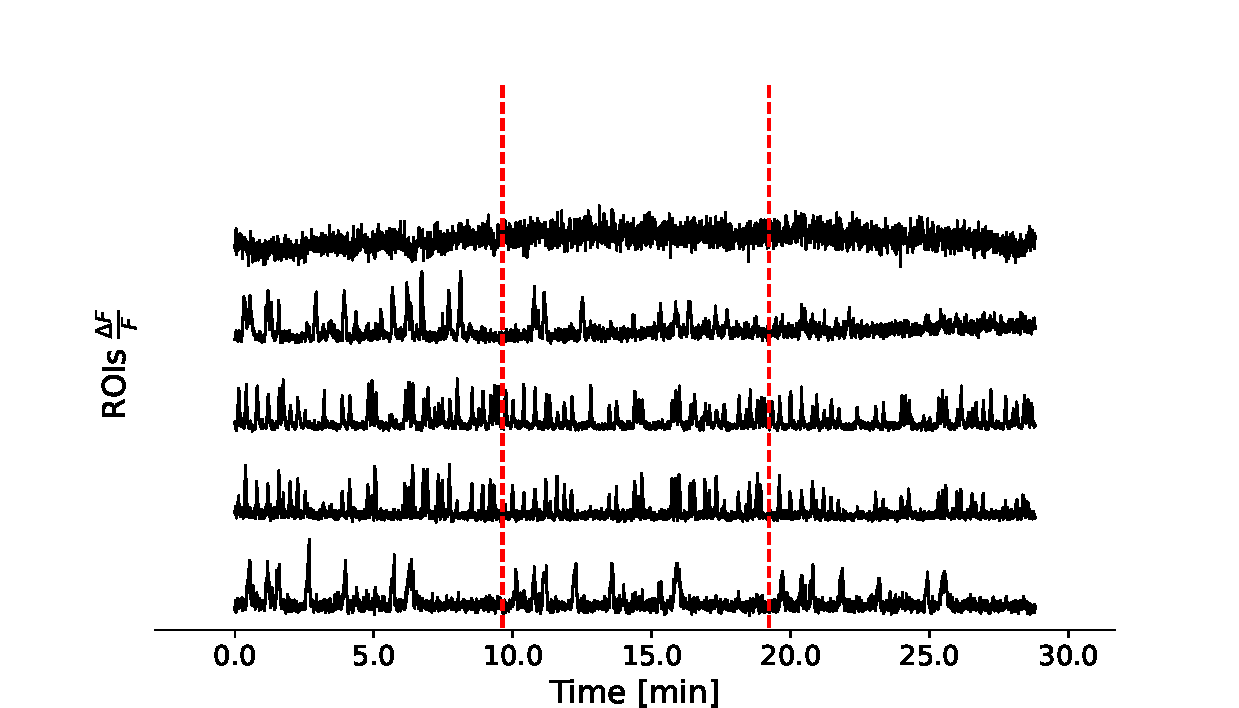
\includegraphics[width=14cm]{figs/autocorrelation.pdf}
    \end{tikzfigure} 
    \end{minipage} 
    \vspace{0.6}

    \textbf{2. Direction selective ROIs:} next Step was 
    to search for ROIs that correlated with a direction selective regressor (1 for clockwise / counter, else is 0)
    
    \begin{minipage}{0.08\textwidth}
        \begin{tikzfigure}[]
            \label{Rois}
            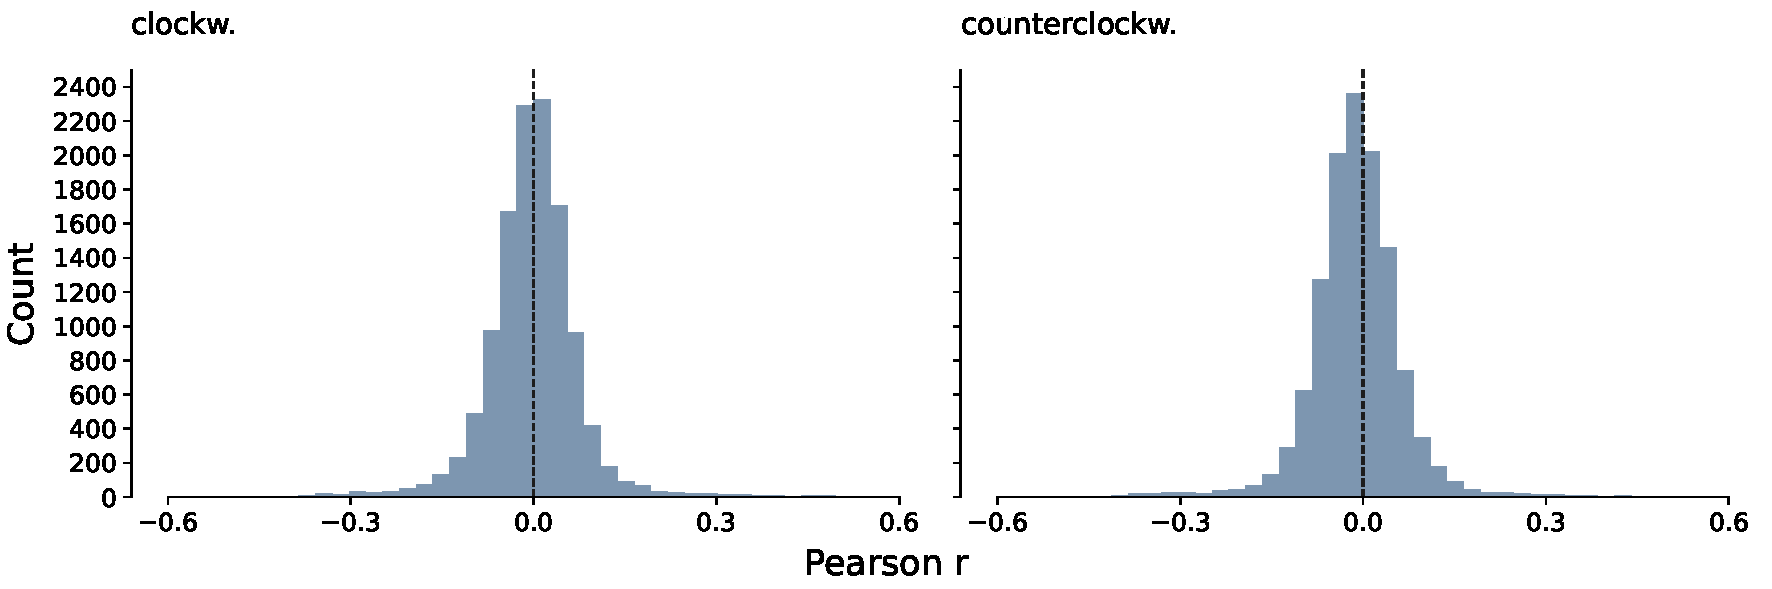
\includegraphics[width=10cm]{figs/directioncorrelation.pdf}
        \end{tikzfigure} 
        \end{minipage}
        \begin{minipage}{0.24\textwidth}
        \begin{tikzfigure}[]
            \label{Raw}
            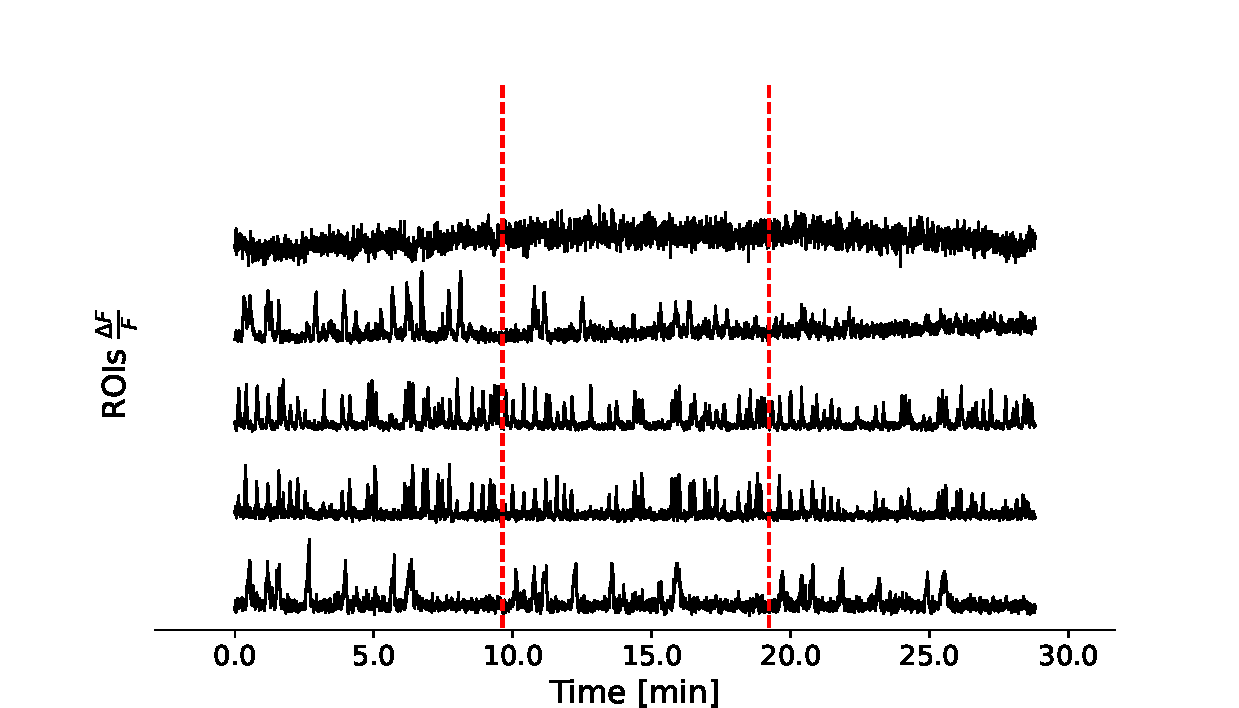
\includegraphics[width=14cm]{figs/autocorrelation.pdf}
        \end{tikzfigure} 
        \end{minipage} 

    }

\column{0.6666}
\myblock[MyBlock]{Motion blindness calcium data vs behaviour}{
        \begin{multicols*}{2}
          \textbf{Calcium}
          1. Stimulus

          \vfill
          \null
          \columnbreak
        \textbf{Bahviour}
        \begin{tikzfigure}[]
            \label{Raw}
            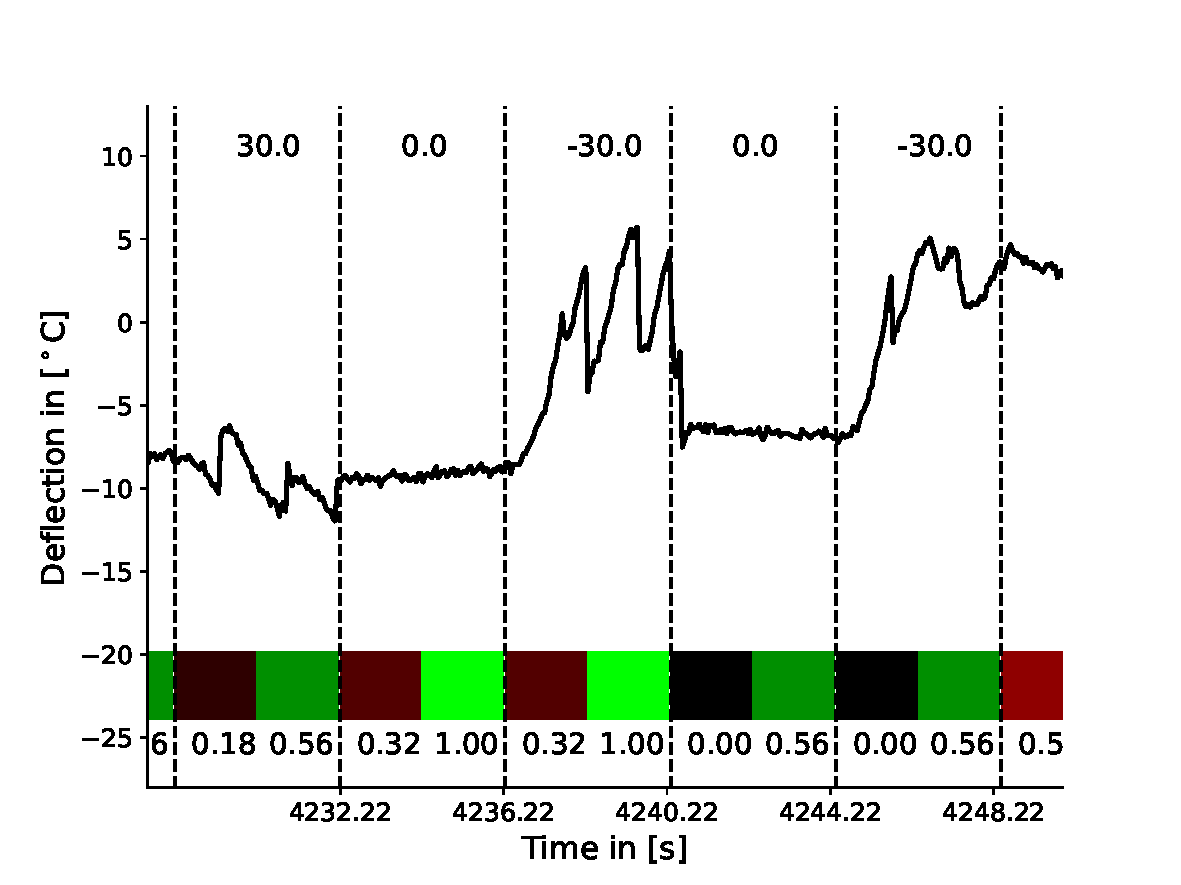
\includegraphics[width=20cm]{figs/eyestimulus.pdf}
        \end{tikzfigure} 
        \end{multicols*}



}

\myblock[MyBlock]{Interactions at modulations}{
    \vspace{-1.2cm}
    \begin{tikzfigure}[]
        \label{modulations}
        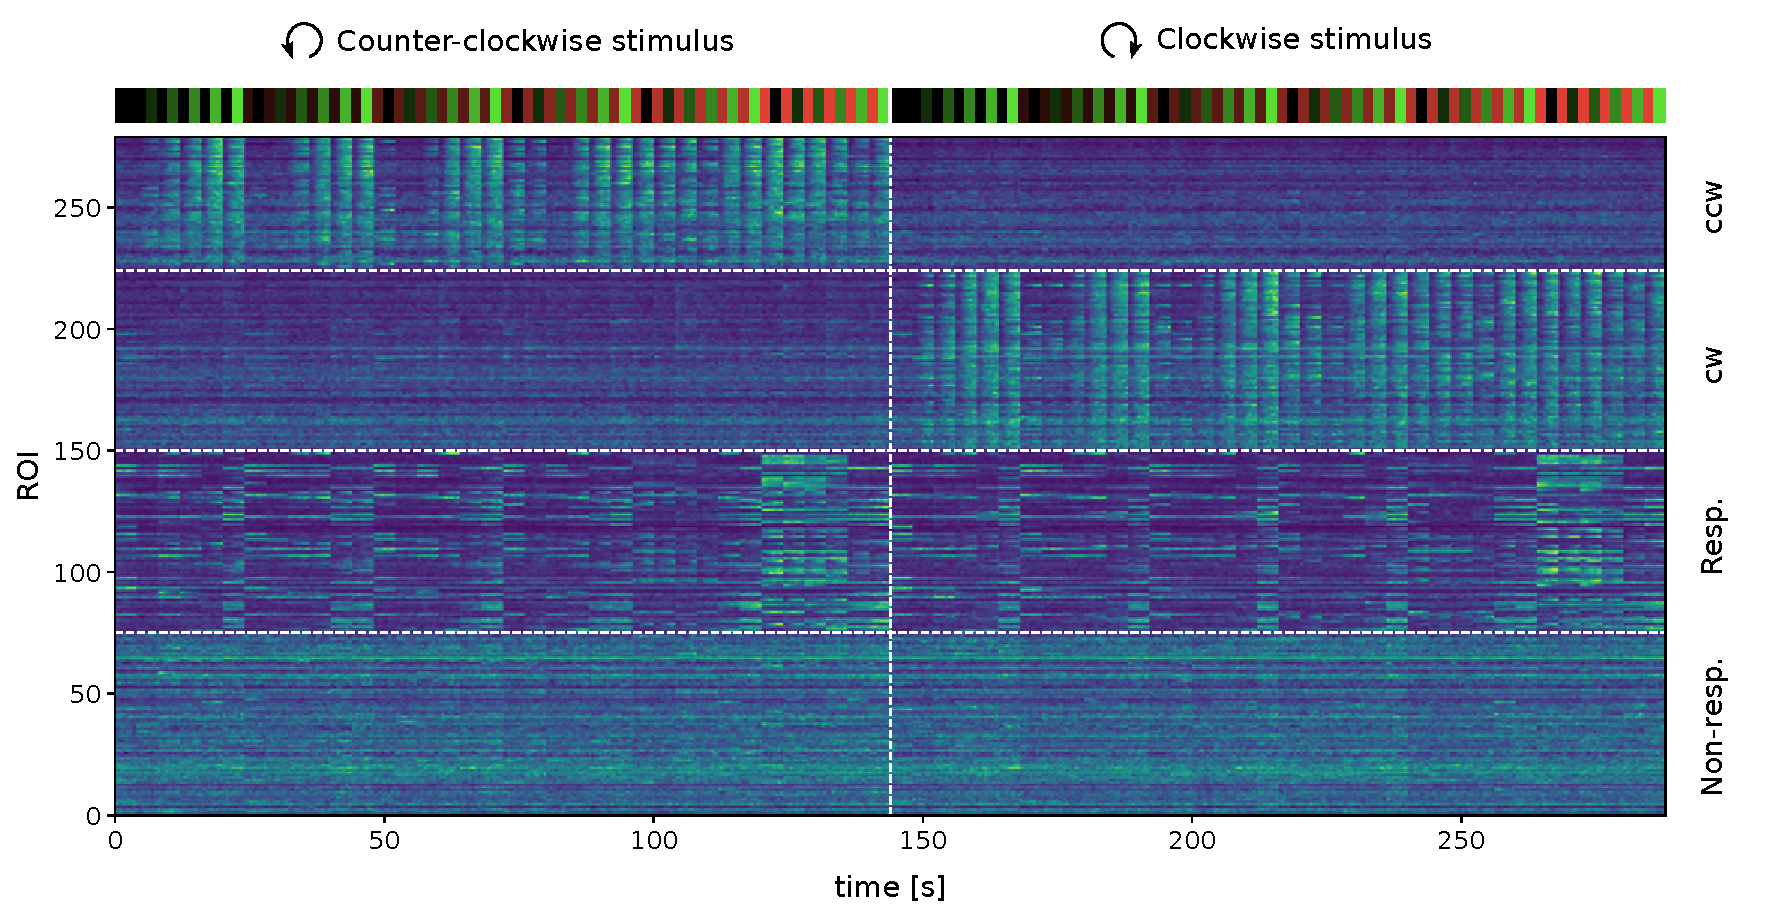
\includegraphics[width=\linewidth]{figs/testimg.pdf
        }
    \end{tikzfigure}

    \begin{multicols}{2}
        \begin{itemize}
            \setlength\itemsep{0.5em}
            \item $\Delta$EOD$f$ does not appear to decrease during synchronous modulations (\textbf{A}).
            \item Individuals that rise their EOD$f$ first appear to rise their frequency higher compared to reactors (\textbf{B}).
            \vfill
            \null
            \columnbreak
            \item Synchronized fish keep distances below 1 m (\textbf{C}) but distances over 3 m also occur (see \textbf{movie}).
            \item Spatial interactions increase \textbf{after} the start of a synchronous modulation (\textbf{D}).
        \end{itemize}
    \end{multicols}
    \vspace{-1cm}
}

\myblock[MyBlock]{Conclusion}{
    \begin{itemize}
        \setlength\itemsep{0.5em}
        \item Our analysis is the first to indicate that \textit{A. leptorhynchus} uses long, diffuse and synchronized EOD$f$ signals to communicate in addition to chirps and rises.
        \item The recorded fish do not exhibit jamming avoidance behavior while close during synchronous modulations.
        \item Synchronous signals \textbf{initiate} spatio-temporal interactions.
    \end{itemize}
    \vspace{0.2cm}
    }
\end{columns}

\node [above right, text=white, outer sep=45pt,minimum width=\paperwidth, align=center, draw, fill=unired, color=unired] at (-43.6,-61) { \textcolor{white}{\normalsize Contact: patrick.weygoldt@student.uni-tuebingen.de}};

\end{document}